\section{Introduction}
    
    
	
    % In computer vision, the task of class-agnostic object tracking is challenging since no target-specific model can be learnt \emph{a priori} and yet the model has to handle target appearance changes, varying lighting conditions and occlusion. 
    In computer vision, designing an algorithm for model-free tracking of anonymous objects is challenging, since no target-specific information can be gathered \emph{a priori} and yet the algorithm has to handle target appearance changes, varying lighting conditions and occlusion. 
    To make it even more difficult, the tracked object often constitutes but a small fraction of the visual field. 
    The remaining parts may contain \emph{distractors}, which are visually salient objects resembling the target but hold no relevant information. 
    Despite this fact, recent models often process the whole image,
    % exposing them to noise 
    which exposes them to noise
    and increases the associated computational cost or they use heuristic methods to decrease the size of search regions. 
    This in contrast to human visual perception, which does not process the visual field in its entirety, but rather acknowledges it briefly and focuses on processing small fractions thereof, which we dub \emph{visual attention}.
    
    
\begin{figure}[ht!]
	\centering
	\begin{minipage}[c]{0.67\textwidth}
		\centering
        \begin{subfigure}[b]{1.\textwidth}
      		 \centering
             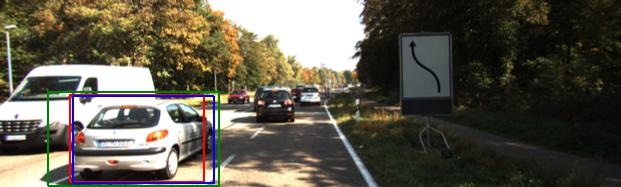
\includegraphics[width=\textwidth]{HART/att_img}
        \end{subfigure}
%        \hspace{-30pt}
        \begin{minipage}{.85\textwidth}
        	\centering
            \begin{subfigure}[b]{.29\textwidth}
                \sidecaption{fig:glimpse}
                \raisebox{-.5\height}{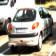
\includegraphics[width=\textwidth, cfbox=darkgreen 1pt 0pt]{HART/att_glimpse}}
            \end{subfigure}
            \hfill
            \hspace{8pt}
            \begin{subfigure}[b]{.29\textwidth}
                \sidecaption{fig:mask}
                \raisebox{-.5\height}{
\includegraphics[width=\textwidth]{HART/att_mask}}
            \end{subfigure}
            \hfill
            \hspace{5pt}
            \begin{subfigure}[b]{.29\textwidth}
                \sidecaption{fig:overlay}
                \raisebox{-.5\height}{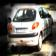
\includegraphics[width=\textwidth]{HART/att_overlay}}
            \end{subfigure}
        \end{minipage}
	\end{minipage}
	\begin{minipage}[c]{0.2\textwidth}
   		\caption{KITTI image with the \textcolor{blue}{ground-truth} and \textcolor{red}{predicted} bounding boxes and an \textcolor{darkgreen}{attention glimpse}. The lower row corresponds to the hierarchical attention of our model: $1^{st}$ layer extracts an attention glimpse (a), the $2^{nd}$ layer uses appearance attention to build a location map (b). The $3^{rd}$ layer uses the location map to suppress distractors, visualised in (c).}
        \label{fig:img_with_att}
	\end{minipage}
\end{figure}
    
    
    %%% Neural attention mechanisms are cool and widely studied in CV and neuroscience
    Attention mechanisms have recently been explored in machine learning in a wide variety of contexts \cite{Vinyals2014, Jaderberg2015}, often providing new capabilities to machine learning algorithms \cite{Graves2016,Wierstra2015draw, Eslami2016}. While they improve efficiency \cite{Graves2014recurrent} and performance on state-of-the-art machine learning benchmarks \cite{Vinyals2014}, their architecture is much simpler than that of the mechanisms found in the human visual cortex \cite{Dayan2001}. Attention has also been long studied by neuroscientists \cite{Ungerleider2000}, who believe that it is crucial for visual perception and cognition \cite{Olshausen2016foveal}, since it is inherently tied to the architecture of the visual cortex and can affect the information flow inside it. Whenever more than one visual stimulus is present in the receptive field of a neuron, all the stimuli compete for computational resources due to the limited processing capacity. 
	%%% How attention is relevant to tracking in cv
	% 	Types of attention
	Visual attention can lead to suppression of distractors by reducing the size of the receptive field of a neuron and by increasing sensitivity at a given location in the visual field (\emph{spatial attention}). It can also amplify activity in different parts of the cortex, which are
	specialised in processing different types of features, leading to  response enhancement with respect to those features (\emph{appearance attention}).
% 	Distinct pathways
	The functional separation of the visual cortex is most apparent in two distinct processing pathways. After leaving the eye, the sensory inputs enter the primary visual cortex (known as \emph{V1}) and then split into the \emph{dorsal stream}, responsible for estimating spatial relationships (\emph{where}), and the \emph{ventral stream}, which targets appearance-based features (\emph{what}).

    Inspired by the general architecture of the human visual cortex and the role of attention mechanisms, this work presents a biologically-inspired recurrent model for single object tracking in videos (\emph{cf.} \cref{sec:att}). Tracking algorithms typically use simple motion models and heuristics to decrease the size of the search region. It is interesting to see whether neuroscientific insights can aid our computational efforts, thereby improving the efficiency and performance of single object tracking.
    % 	Inspired by the general architecture of the human visual cortex and the role of attention mechanisms, this work presents a biologically-inspired recurrent model for single object tracking in videos (\emph{cf.} \cref{sec:att}).
	% 	Different sources of attention
	It is worth noting that visual attention can be induced by the stimulus itself (due to, \eg high contrast) in a \emph{bottom-up} fashion or by back-projections from other brain regions and working memory as \emph{top-down} influence. The proposed approach exploits this property to create a feedback loop that steers the \emph{three} layers of visual attention mechanisms in our hierarchical attentive recurrent tracking (\emph{HART}) framework, see \Cref{fig:img_with_att}. The first stage immediately discards spatially irrelevant input, while later stages focus on producing target-specific filters to emphasise visual features \emph{particular} to the object of interest.
	
% 	By factoring the problem into its constituent parts, we arrive at a familiar statistical domain; namely that of maximum likelihood estimation (MLE). 
    The resulting framework is end-to-end trainable and we resort to maximum likelihood estimation (MLE) for parameter learning.
	This follows from our interest in estimating the distribution over object locations in a sequence of images, given the initial location from whence our tracking commenced. 
	Formally, given a sequence of images $\bxTs \in \RR^{H \times W \times C}$, where the superscript denotes height, width and the number of channels of the image, respectively, and an initial location for the tracked object given by a bounding box $\bb_1 \in \RR^4$, the conditional probability distribution factorises as
    \begin{equation}
        \p{\bb_{2:T}}{\bxTs, \bb_1} = \int \p{\B{h}_1}{\bx_1, \bb_1} \prod_{t=2}^T \int \p{\bbt}{\B{h}_t} \p{\B{h}_t}{\bxt, \bb_{t-1}, \B{h}_{t-1}} \dint \B{h}_t \dint \B{h}_1,
    \end{equation}
    where we assume that motion of an object can be described by a Markovian state $\B{h}_t$.
    Our bounding box estimates are given by $\widehat{\bb}_{2:T}$, found by the MLE of the model parameters. In sum, our contributions are threefold: 
    Firstly, a hierarchy of attention mechanisms that leads to suppressing distractors and computational efficiency is introduced.
    Secondly, a biologically plausible combination of attention mechanisms and recurrent neural networks is presented for object tracking.
    Finally, our attention-based tracker is demonstrated using real-world sequences in challenging scenarios where previous recurrent attentive trackers have failed.
    
    \iffalse
    \begin{itemize}
        \item a biologically plausible way of combining attention mechanisms with recurrent neural networks for object tracking,
        \item a hierarchy of attention mechanisms that leads to suppressing distractors and computational efficiency,
        \item the scaling of an attention-based tracker to real-world exceeding prior recurrent attentive tracking models. 
    \end{itemize}
    \fi
    
    Next we briefly review related work (\Cref{sec:background}) before describing how information flows through the components of our hierarchical attention in \Cref{sec:att}. \Cref{sec:loss} details the losses applied to guide the attention. \Cref{sec:exp} presents experiments on KTH and KITTI datasets with comparison to related attention-based trackers. \Cref{sec:discussion} discusses the results and intriguing properties of our framework and \Cref{sec:conclusion} concludes the work. Code and results are available online\footnote{\url{https://github.com/akosiorek/hart}}.
        

	
	
	
	
	
	
	
	
	

	